%%%%%%%%%%%%%%%%%%%%%%%%%%%%%%%%%%%%%%%%%%%%%%%%%%%%%%%%%%%%%%%%%%%%%%%%%%%%%%%%
%% Plantilla de memoria en LaTeX para la ETSIT - Universidad Rey Juan Carlos
%%
%% Por Gregorio Robles <grex arroba gsyc.urjc.es>
%%     Grupo de Sistemas y Comunicaciones
%%     Escuela Técnica Superior de Ingenieros de Telecomunicación
%%     Universidad Rey Juan Carlos
%% (muchas ideas tomadas de Internet, colegas del GSyC, antiguos alumnos...
%%  etc. Muchas gracias a todos)
%%
%% La última versión de esta plantilla está siempre disponible en:
%%     https://github.com/gregoriorobles/plantilla-memoria
%%
%% Para obtener PDF, ejecuta en la shell:
%%   make
%% (las imágenes deben ir en PNG o JPG)

%%%%%%%%%%%%%%%%%%%%%%%%%%%%%%%%%%%%%%%%%%%%%%%%%%%%%%%%%%%%%%%%%%%%%%%%%%%%%%%%

\documentclass[a4paper, 12pt]{book}
\usepackage[T1]{fontenc}

\usepackage[a4paper, left=2.5cm, right=2.5cm, top=3cm, bottom=3cm]{geometry}
\usepackage{times}
\usepackage[utf8]{inputenc}
%\usepackage[latin-1]{inputenc}
\usepackage[spanish]{babel} % Comenta esta línea si tu memoria es en inglés
\usepackage{url}
%\usepackage[dvipdfm]{graphicx}
\usepackage{graphicx}
\usepackage{float}  %% H para posicionar figuras
\usepackage[nottoc, notlot, notlof, notindex]{tocbibind} %% Opciones de índice
\usepackage{latexsym}  %% Logo LaTeX
\usepackage{pdfpages}

\usepackage{hyperref}

\title{Memoria del Proyecto Fin de Carrera "Conference Book Generator"}
\author{Seila Oliva Muñoz}

\renewcommand{\baselinestretch}{1.5}  %% Interlineado

\begin{document}

\renewcommand{\refname}{Bibliografía}  %% Renombrando
\renewcommand{\appendixname}{Apéndice}

%%%%%%%%%%%%%%%%%%%%%%%%%%%%%%%%%%%%%%%%%%%%%%%%%%%%%%%%%%%%%%%%%%%%%%%%%%%%%%%%
% PORTADA

\begin{titlepage}
\begin{center}
\begin{tabular}[c]{c c}
%
\includegraphics[bb=0 0 194 352, scale=0.25]{logo} &

\includegraphics[scale=0.25]{img/logo_vect.png} &
\begin{tabular}[b]{l}
\Huge
\textsf{UNIVERSIDAD} \\
\Huge
\textsf{REY JUAN CARLOS} \\
\end{tabular}
\\
\end{tabular}

\vspace{3cm}

\Large
GRADO DE INGENIERÍA EN TECNOLOGÍAS DE LA TELECOMUNICACIÓN

\vspace{0.4cm}

\large
Curso Académico 2017/2018

\vspace{0.8cm}

Trabajo Fin de Grado

\vspace{2.5cm}

\LARGE
CONFERENCE BOOK GENERATOR

\vspace{4cm}

\large
Autor : Seila Oliva Muñoz \\
Tutor : Dr. Gregorio Robles
\end{center}
\end{titlepage}

\newpage
\mbox{}
\thispagestyle{empty} % para que no se numere esta pagina


%%%%%%%%%%%%%%%%%%%%%%%%%%%%%%%%%%%%%%%%%%%%%%%%%%%%%%%%%%%%%%%%%%%%%%%%%%%%%%%%
%%%% Para firmar
\clearpage
\pagenumbering{gobble}
\chapter*{}

\vspace{-4cm}
\begin{center}
\LARGE
\textbf{Trabajo Fin de Grado}

\vspace{1cm}
\large
Conference Book Generator

\vspace{1cm}
\large
\textbf{Autor :} Seila Oliva Muñoz \\
\textbf{Tutor :} Dr. Gregorio Robles Martínez

\end{center}

\vspace{1cm}
La defensa del presente Proyecto Fin de Carrera se realizó el día \qquad$\;\,$ de \qquad\qquad\qquad\qquad \newline de 2018, siendo calificada por el siguiente tribunal:


\vspace{0.5cm}
\textbf{Presidente:}

\vspace{1.2cm}
\textbf{Secretario:}

\vspace{1.2cm}
\textbf{Vocal:}


\vspace{1.2cm}
y habiendo obtenido la siguiente calificación:

\vspace{1cm}
\textbf{Calificación:}


\vspace{1cm}
\begin{flushright}
Fuenlabrada, a \qquad$\;\,$ de \qquad\qquad\qquad\qquad de 2018
\end{flushright}

%%%%%%%%%%%%%%%%%%%%%%%%%%%%%%%%%%%%%%%%%%%%%%%%%%%%%%%%%%%%%%%%%%%%%%%%%%%%%%%%
%%%% Dedicatoria

\chapter*{}
\pagenumbering{Roman} % para comenzar la numeracion de paginas en numeros romanos
\begin{flushright}
\textit{Dedicado a \\
mi familia / mi abuelo / mi abuela}
\end{flushright}

%%%%%%%%%%%%%%%%%%%%%%%%%%%%%%%%%%%%%%%%%%%%%%%%%%%%%%%%%%%%%%%%%%%%%%%%%%%%%%%%
%%%% Agradecimientos

\chapter*{Agradecimientos}
%\addcontentsline{toc}{chapter}{Agradecimientos} % si queremos que aparezca en el índice
\markboth{AGRADECIMIENTOS}{AGRADECIMIENTOS} % encabezado

Aquí vienen los agradecimientos\ldots Aunque está bien acordarse de la pareja, no hay que olvidarse de dar las gracias a tu madre, que aunque a veces no lo parezca disfrutará tanto de tus logros como tú\ldots
Además, la pareja quizás no sea para siempre, pero tu madre sí.

%%%%%%%%%%%%%%%%%%%%%%%%%%%%%%%%%%%%%%%%%%%%%%%%%%%%%%%%%%%%%%%%%%%%%%%%%%%%%%%%
%%%% Resumen

\chapter*{Resumen}
%\addcontentsline{toc}{chapter}{Resumen} % si queremos que aparezca en el índice
\markboth{RESUMEN}{RESUMEN} % encabezado
En la actualidad es muy frecuente la realización de seminarios y conferencias en las que se tratan temas concretos de diferentes índoles, a las que suelen ir personas especializadas en el tema a tratar dispuesta a conocer otras personas que compartan sus mismos intereses, incluso buscando personas con las que trabajar.\\

Es por esto que surge la idea de tener los datos de todos los asistentes para conocer sus intereses y datos de contacto por si interesa una posible colaboración/contratación.\\

Mi proyecto consiste en la elaboración de un \textit{book} en el que aparezcan estos datos de todos los participantes. Para ello, previamente los participantes tendrán que rellenar un formulario de \textit{Google Forms}. Una vez se hayan recopilado los datos de todos los participantes, se trasladarán a una \textit{Google Sheet}, cuya URL se introducirá en el programa que he elaborado con \textbf{\textit{Python}}.\\

Se extraerán los datos de los participantes de esta hoja de cálculo, y se manipularán en caso de que sea necesario para, con ellos, generar un documento en \LaTeX. Este documento se compilará para obtener un PDF en el que aparecerán los datos de todos los asistentes y estará listo para ser impreso en forma de revista.


%%%%%%%%%%%%%%%%%%%%%%%%%%%%%%%%%%%%%%%%%%%%%%%%%%%%%%%%%%%%%%%%%%%%%%%%%%%%%%%%
%%%% Resumen en inglés

\chapter*{Summary}
%\addcontentsline{toc}{chapter}{Summary} % si queremos que aparezca en el índice
\markboth{SUMMARY}{SUMMARY} % encabezado

At present, it is very common to make seminars and conferences that address specific issues of different kinds, where usually go people specialized in the issue whobe willing to meet other people who share their same interests, even looking for people with those that work.\\

This is why the idea of having the data of all the attendees to know their interests and contact data in case a possible collaboration/contracting interests.\\

My project consists in the elaboration of a \textit{book} in which these data of all the participants appear. To do this, previously the participants will have to fill a \textit{Google Forms} form. Once the data of all the participants has been collected, they will be moved to a \textit{Google Sheet}, whose URL will be introduced in the program that I have created with \textbf{Python}.\\

The data of the participants of this spreadsheet will be extracted, and they will be manipulated in case it is necessary to generate a document in \LaTeX with them. This document will be compiled to obtain a PDF in which the data of all the attendees will appear and it will be ready to be printed in the form of a magazine.


%%%%%%%%%%%%%%%%%%%%%%%%%%%%%%%%%%%%%%%%%%%%%%%%%%%%%%%%%%%%%%%%%%%%%%%%%%%%%%%%
%%%%%%%%%%%%%%%%%%%%%%%%%%%%%%%%%%%%%%%%%%%%%%%%%%%%%%%%%%%%%%%%%%%%%%%%%%%%%%%%
% ÍNDICES %
%%%%%%%%%%%%%%%%%%%%%%%%%%%%%%%%%%%%%%%%%%%%%%%%%%%%%%%%%%%%%%%%%%%%%%%%%%%%%%%%

% Las buenas noticias es que los índices se generan automáticamente.
% Lo único que tienes que hacer es elegir cuáles quieren que se generen,
% y comentar/descomentar esa instrucción de LaTeX.

%%%% índice de contenidos
\tableofcontents
%%%% índice de figuras
\cleardoublepage
%\addcontentsline{toc}{chapter}{Lista de figuras} % para que aparezca en el indice de contenidos
\listoffigures % indice de figuras
%%%% índice de tablas
%\cleardoublepage
%\addcontentsline{toc}{chapter}{Lista de tablas} % para que aparezca en el indice de contenidos
%\listoftables % indice de tablas


%%%%%%%%%%%%%%%%%%%%%%%%%%%%%%%%%%%%%%%%%%%%%%%%%%%%%%%%%%%%%%%%%%%%%%%%%%%%%%%%
%%%%%%%%%%%%%%%%%%%%%%%%%%%%%%%%%%%%%%%%%%%%%%%%%%%%%%%%%%%%%%%%%%%%%%%%%%%%%%%%
% INTRODUCCIÓN %
%%%%%%%%%%%%%%%%%%%%%%%%%%%%%%%%%%%%%%%%%%%%%%%%%%%%%%%%%%%%%%%%%%%%%%%%%%%%%%%%

\cleardoublepage
\chapter{Introducción}
\label{chap:intro} % etiqueta para poder referenciar luego en el texto con ~\ref{sec:intro}
\pagenumbering{arabic} % para empezar la numeración de página con números

\section{Motivación}
\label{sec:motivacion}
Hoy en día es muy frecuente la realización de seminarios o conferencias de muy diversos temas. A ellos acude gente de diferentes partes del mundo, con perfiles similares o diferentes, dispuestos a aumentar su lista de contactos. \\

Normalmente, la única manera de conocer gente en estos lugares es presentándose personalmente a cada persona, y en una conferencia con un número grande de personas esta labor puede resultar tediosa, por no decir prácticamente imposible.\\

Por esto, mi tutor, Gregorio, me contó la idea de crear un ``Book'' o revista en el que apareciesen los datos de todos los asistentes a la conferencia, para repartirlo en el lugar, y así tener el contacto de todos. En este libro cada asistente podrá incluir sus datos de contacto, su centro de trabajo, sus intereses, etc.\\

Este proyecto pretende automatizar la labor de hacer este Book, de manera que cada asistente rellene un formulario previamente con sus datos, y que el documento se genere automáticamente.


\section{Estructura de la memoria}
\label{sec:estructura}
Con el fin de facilitar la lectura de la memoria, en esta sección se detalla la estructura de la misma y el contenido que se trata en cada una de las secciones:
\begin{itemize}
  \item \textbf{Capítulo ~\ref{chap:intro} Introducción.} Contexto en el que surge la idea del proyecto y breve explicación de la estructura de la memoria.

  \item \textbf{Capítulo ~\ref{chap:objetivos}: Objetivos.} En esta sección se explican los objetivos marcados durante la realización del proyecto.

  \item \textbf{Capítulo ~\ref{chap:estadoarte}: Estado del arte.} Presentación de las tecnologías con las que se ha desarrollado el proyecto.
  
  \item \textbf{Capítulo ~\ref{chap:diseño}: Diseño e implementación.} Explicación del desarrollo del proyecto paso a paso.

  \item \textbf{Capítulo ~\ref{chap:resultados}: Resultados.} Análisis de los resultados obtenidos.
  
  \item \textbf{Capítulo ~\ref{chap:conclusiones}: Conclusiones.} Conclusiones finales tras la realización del trabajo, como los objetivos conseguidos, posibles mejoras futuras del proyecto, cómo he aplicado lo aprendido en la carrera o lo que he aprendido durante la realización del proyecto.
\end{itemize}



%%%%%%%%%%%%%%%%%%%%%%%%%%%%%%%%%%%%%%%%%%%%%%%%%%%%%%%%%%%%%%%%%%%%%%%%%%%%%%%%
%%%%%%%%%%%%%%%%%%%%%%%%%%%%%%%%%%%%%%%%%%%%%%%%%%%%%%%%%%%%%%%%%%%%%%%%%%%%%%%%
% OBJETIVOS %
%%%%%%%%%%%%%%%%%%%%%%%%%%%%%%%%%%%%%%%%%%%%%%%%%%%%%%%%%%%%%%%%%%%%%%%%%%%%%%%%

\cleardoublepage % empezamos en página impar
\chapter{Objetivos} % título del capítulo (se muestra)
\label{chap:objetivos} % identificador del capítulo (no se muestra, es para poder referenciarlo)

\section{Objetivo general} % título de sección (se muestra)
\label{sec:objetivo-general} % identificador de sección (no se muestra, es para poder referenciarla)
El objetivo de este proyecto es crear un recurso para que todas las personas que asistan a una conferencia/seminario puedan conocer al resto de asistentes, así como darse a conocer ellos mismos, y de esta forma poder obtener información sobre cada uno (datos de contacto, situación laboral \ldots).\\

Para ello, se persigue otro objetivo que es automatizar esta labor: crear un programa que sea capaz de tomar como entrada los datos de cada asistente y generar un documento con toda la información.


\section{Objetivos específicos}
\label{sec:objetivos-especificos}
Los objetivos específicos que llevé a cabo a lo largo del proyecto fueron los siguientes:
\begin{itemize}
  \item \textbf{Usar la aplicación para casos reales.} Utilizar la aplicación para generar \textit{books} para conferencias reales, imprimirlos y que se repartan en ellas.
  \item \textbf{Sencillez de uso.} Intentar que la aplicación se pueda ejecutar tanto por personas que están familiarizadas con las tecnologías utilizadas, como por las que no las conocen o no saben mucho sobre ellas.
\end{itemize}

\section{Planificación temporal}
\label{sec:planificacion-temporal}
La realización de este proyecto me ha ocupado todo un curso académico (9 meses), y las fases que he seguido han sido las siguientes:
\begin{itemize}
	\item \textbf{Idea de proyecto.} En primer lugar, me reuní con mi tutor del proyecto, Gregorio, para que me ayudase a elegir un proyecto que se adaptase a lo que estaba buscando. Una vez decidido el proyecto, tomé un tiempo para estudiarlo y saber qué tecnologías iba a necesitar para su desarrollo.
	\item \textbf{Aprendizaje de las tecnologías utilizadas.} Una vez me di cuenta de las tecnologías necesarias, comencé por aprender sobre ellas: para qué sirven, cómo utilizarlas \ldots Este proceso es imprescindible para la continuación del proyecto.
	\item \textbf{Desarrollo del proyecto.} Desarrollo del código en Python para conseguir las ideas anteriormente expuestas.
	\item \textbf{Redacción de la memoria.} Como último paso del proyecto, comencé a escribir esta memoria en la que se recopilan en detalle todos los pasos que seguí para la consecución del proyecto.
\end{itemize}


%%%%%%%%%%%%%%%%%%%%%%%%%%%%%%%%%%%%%%%%%%%%%%%%%%%%%%%%%%%%%%%%%%%%%%%%%%%%%%%%
%%%%%%%%%%%%%%%%%%%%%%%%%%%%%%%%%%%%%%%%%%%%%%%%%%%%%%%%%%%%%%%%%%%%%%%%%%%%%%%%
% ESTADO DEL ARTE %
%%%%%%%%%%%%%%%%%%%%%%%%%%%%%%%%%%%%%%%%%%%%%%%%%%%%%%%%%%%%%%%%%%%%%%%%%%%%%%%%

\cleardoublepage
\chapter{Estado del arte}
\label{chap:estadoarte} % identificador del capítulo (no se muestra, es para poder referenciarlo)

En esta sección, se describen las tecnologías utilizadas para la realización del proyecto:

\section{Python}
\label{sec:python}
Python~\cite{python:1} es un lenguaje de programación que busca la simplicidad y facilidad, así como la legibilidad del código. Es un lenguaje interpretado, es decir, no necesita ser compilado para ejecutar.\\

Fue creado en los finales de los ochenta por Guido Can Rossum en el Centro para las Matemáticas y la Informatica (CWI, Centrum Wiskunde \& Informatica), en los Países Bajos. El nombre del lenguaje proviene de la afición de su creador por el grupo de humoristas británicos \textit{Monty Python}.\\

Con Python se pueden hacer todo tipo de programas. Aunque no es un lenguaje específico para el desarrollo web, sí se pueden desarrollar páginas con él.\\

Es un lenguaje multiparadigma: permite más de un estilo de programación (orientada a objetos, imperativa, funcional \ldots). También es multiplataforma, por lo que se puede usar con distintos sistemas informáticos.\\

Una ventaja de Python es que cuenta con un gran número de funciones incorporadas en el lenguaje (por ejemplo, para tratar \emph{strings}, ficheros\ldots) y librerías para usos específicos que podemos importar a nuestro programa, lo que nos ayuda a realizar muchas tareas sin necesidad de programarlas desde cero.\\

Phyton es ideal para trabajar con grandes volúmenes de datos, porque favorece su extracción y procesamiento, siendo el elegido por las empresas de Big Data. A nivel científico, posee una amplia biblioteca de recursos con especial énfasis en las matemáticas.


\subsection{Python 2 y Python 3}
\label{python2y3}
Hay dos versiones principales de Python: Python 2 y Python 3. Python 2 ha estado presente durante mucho tiempo, por lo que es la versión más extendida actualmente y la que tiene mayor disponibilidad de bibliotecas. La versión más popular de Python 2 es Python 2.7.\\

Sin embargo, Python 3 se considera el futuro de Python, ya que está pensado para añadir más características y corregir errores anteriores, y está en continuo desarrollo. Mientras, Python 2 no añadirá ya prácticamente nuevas características. Por ello, Python 3 comienza a adelantar a Python 2, en lo que a usuarios que la usan se refiere.\\

Las funcionalidades de Python 2 y 3 son, en su mayoría, iguales, pero hay algunas diferencias en la sintaxis y la manipulación. Las principales diferencias entre estas dos versiones son:
\begin{itemize}
	\item \textbf{Print:} quizá es la diferencia más destacada a simple vista, y es que \textit{print} ha pasado de ser una sentencia a ser una función. Esto se traduce, sobre todo, a que con Python 2 se puede escribir \verb"print 'Hello World'" , sin necesidad de paréntesis. En cambio, en Python 3 es obligatorio el uso de paréntesis para hacer un \textit{print}: \verb"print('Hello World')".
	\item \textbf{División entera}: en Python 2 la división de dos números enteros da como resultado un número entero (3/2 = 1), y para que el resultado tenga decimales hay que escribir dividendo y divisor en forma de decimal (3.0/2.0 = 1.5). En Python 3 la división de enteros ya da como resultado un número decimal (3/2 = 1.5).
	\item \textbf{Soporte Unicode:} para hacer una cadena Unicode en Python 2, se debe añadir el caracter \textit{'u'} a la cadena: \verb"u'Hello World'", mientras que en Python 3 las cadenas son Unicode por omisión.
	\item \textbf{Next (iterables):} en Python 2, para obtener el siguiente elemento de un iterador, se pueden usar tanto el método iter\textbf{.next()} como la función \textbf{next}(iter). Sin embargo, en Python 3 sólo se puede utilizar la función.
	\item \textbf{Input:} en Python 2 hay dos funciones para introducir datos por teclado: \textit{raw\_input()} (los datos introducidos los trata como una cadena de texto) e \textit{input()} (los datos introducidos los trata por su tipo, es decir, si introducimos 15 lo trata como un int). En Python 3 se ha eliminado la función \textit{raw\_input()}, y en su lugar permanece la función \textit{input()} con las características del \textit{raw\_input()} de Python 2.
\end{itemize}



\section{\LaTeX}
\label{sec:latex}
\LaTeX~\cite{latex:1} es un sistema de composición de textos (de software libre), orientado especialmente a la creación de libros y documentos científicos y técnicos que contengan fórmulas matemáticas. Está formado por un gran conjunto de macros de \TeX, con la intención de facilitar el uso del lenguaje de composición tipográfica, \TeX.\\

Una de las ventajas de \LaTeX es la calidad profesional de los documentos que genera, así como su excelente calidad de imprenta. Otra ventaja es que permite separar claramente el contenido y el formato del documento.\\

\LaTeX presupone una filosofía de trabajo diferente a la de los procesadores de texto habituales (``lo que ves es lo que obtienes'') y se basa en instrucciones. Tradicionalmente, este aspecto se ha considerado una desventaja. Sin embargo, \LaTeX permite a quien escribe un documento centrarse exclusivamente en el contenido, sin tener que preocuparse de los detalles del formato.\\

El proceso de generación de un documento con \LaTeX consiste en 3 pasos:
\begin{itemize}
	\item \textbf{Editar.} El primer paso es usar un editor para generar un archivo con extensión \textit{.tex}, y en él escribir el código \LaTeX que describa la estructura y contenido del documento.
	\item \textbf{Compilar.} Compilar es el proceso realizado por el motor de \LaTeX, que convierte los archivos \textit{.tex} en documentos con formato \textit{.pdf}, que se podrán imprimir y ver en pantalla. El proceso de compilación detectará e indicará los errores que tenga el código, que habrá que corregir y volver a compilar para obtener el documento \textit{.pdf}.
	\item \textbf{Visualizar.} Una vez compilado, y sin errores, podremos visualizar el resultado. Hay editores específicos para \LaTeX que permiten compilar y visualizar el documento desde el propio editor; si no fuese el caso, habría que dirigirse al directorio para buscar y abrir el archivo \textit{.pdf} que ha sido generado.
\end{itemize}

\subsection{Creación de un documento \LaTeX}
\label{crearLatex}
Un documento \LaTeX tiene dos partes principales: el preámbulo y el cuerpo del documento.
\begin{itemize}
	\item \textbf{Preámbulo.} Comienza por la instrucción \textit{\textbackslash documentclass[.]\{.\}}. En todas las instrucciones, entre [] se incluyen los parámetros opcionales, que en el caso del \textit{documentclass} son el tamaño de letra (11pt, 12pt\ldots), si el texto va a dos columnas (twocolumn) o ajuste de los márgenes para imprimir a doble cara (twoside). Entre \{\} se incluyen los parámetros obligatorios, que en este caso es el tipo de documento que estamos elaborando (article, report, book\ldots).\\
	En el preámbulo se pueden incluir instrucciones para activar paquetes que agregan funciones adicionales a \LaTeX, así como datos generales sobre el documento que se está escribiendo. Y al final se incluyen los campos \textit{\textbackslash title, \textbackslash author} y \textit{\textbackslash date}, que especifican los datos que irán en el encabezado del documento.\\
	Se puede ver un ejemplo de preámbulo en la Figura ~\ref{fig:preambulo}.
	\begin{figure}[h!]
		\centering
		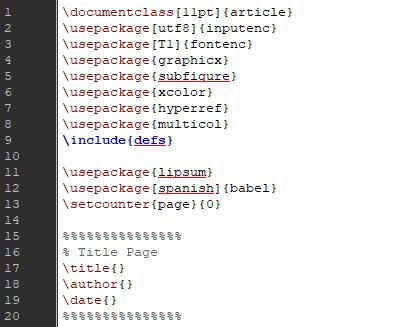
\includegraphics[width=8cm, keepaspectratio]{img/preambulo_latex}
		\caption{Ejemplo de preámbulo}
		\label{fig:preambulo}
	\end{figure}
	
	\item \textbf{Cuerpo del documento.} Está delimitado por los comandos \textit{\textbackslash begin\{document\}} y \textit{\textbackslash end\{document\}}. Si comenzamos el cuerpo con el comando \textit{\textbackslash maketitle} se escribirán los datos del título con la información que se indicó en el preámbulo (título, autor y fecha).\\
	Lo único que queda es empezar a escribir el texto, y \LaTeX se encargará del formato y apariencia. Algunas cosas importantes a tener en cuenta son: 
	\begin{itemize}
		\item \textbf{Signos especiales:} Algunos símbolos no aparecen en el pdf tal cual los escribimos en el editor en el \textit{.tex}, y hay que escribirlos de manera especial, como los signos de apertura de interrogación y exclamación (?` y !`) que habría que escribir ? y ! seguido de un acento grave para que se visualicen correctamente; o las comillas que, tanto para simples como para dobles, para abrirlas hay que escribir acento grave y para cerrarlas comilla simple.
		\item \textbf{Comandos para formato de texto:} hay comandos para títulos y secciones (\mbox{\textit{\textbackslash chapter\{\}}}, \textit{\textbackslash section\{\}}, \textit{\textbackslash subsection\{\}}\ldots) y para enfatizar o cambiar el formato del texto (\textbf{\textbackslash textbf\{\}}, \textit{\textbackslash textit\{\}}, \textsc{\textbackslash textsc\{\}}, \textsf{\textbackslash textsf\{\}}, \textsl{\textbackslash textsl\{\}}, \texttt{\textbackslash texttt\{\}}\ldots).
		\item \textbf{Índice:} \LaTeX genera el índice del documento automáticamente si añadimos la instrucción \textbackslash tableofcontents.
	\end{itemize}
	
	Se puede ver un ejemplo del cuerpo del documento en la Figura ~\ref{fig:cuerpo}.	
	
	\begin{figure}[h!]
		\centering
		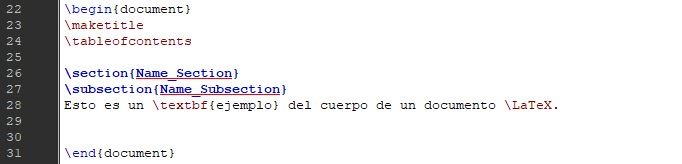
\includegraphics[width=13cm, keepaspectratio]{img/cuerpo_latex}
		\caption{Ejemplo de cuerpo del documento}
		\label{fig:cuerpo}
	\end{figure}
	
\end{itemize}

\subsection{XeTeX}
\label{xetex}
Aunque \LaTeX proporcinoa un amplio conjunto de fuentes, es posible que se desee utilizar una fuente externa que nos guste más, y que esté instalada previamente en el sistema. Esto es posible gracias a XeTeX~\cite{xetex:1}, que es un motor de tipografía \TeX que utiliza Unicode y es compatible con tecnologías de fuentes modernas como OpenType (OTF), TrueType (TTF), Graphite y Apple Advanced Typography (AAT). El compilador necesario es XeTeX o XeLaTeX.\\

En este proyecto, estamos compilando con \textbf{XeLaTeX}.



\section{Google Forms}
\label{sec:googleforms}
Google Forms~\cite{forms:1} es una herramienta útil que permite planificar eventos, enviar una encuesta, hacer preguntas o recopilar otro tipo de información de forma fácil y sencilla.\\

Crear un formulario es tan fácil como añadir las preguntas seleccionando en cada uno el tipo que mejor se adapte a nuestras necesidades. Los tipos de pregunta que nos podemos encontrar son, por ejemplo, texto, tipo test, elegir de listas, desplegables, etc. También permite añadir imágenes, vídeos o saltos de página para dividir la encuesta en secciones.\\

Una vez enviado el formulario a los destinatarios, se irán recopilando las respuestas recibidas. Éstas se pueden guardar en el propio Google Forms, de manera que se mostrarán como un resumen de las respuestas, o se pueden exportar a una hoja de cálculo en la que cada línea estarán las respuestas de cada persona (cada respuesta en una columna).


\section{Google Sheets API}
\label{sec:googlesheet}
Google Sheets API~\cite{sheet:1} permite leer y modificar cualquier aspecto de una hoja de cálculo. La API ofrece dos formas principales de interactuar con la hoja de cálculo:
\begin{itemize}
	\item Leer o escribir solo valores de celdas (con la colección \textit{spreadsheets.values}).
	\item Leer o escribir cualquier aspecto de la hoja de cálculo (con la colección \textit{spreadsheets}).
\end{itemize}

En nuestro caso, es suficiente con la lectura de los valores de las celdas, por lo que usaremos la colección \textbf{spreadsheets.values}\footnote{\url{https://forward2.herokuapp.com/developers/sheets/api/reference/rest/v4/spreadsheets.values?hl=es-419}}.\\

Todos los métodos de la API requieren un parámetro \textit{spreadsheetId} que se utiliza para identificar la hoja de cálculo a la que se accederá. Este ID es el valor entre \textit{``/d/''} y \textit{``/edit''} de la URL de la hoja de cálculo. Esta URL también contiene el \textit{sheetId}, que es el ID de la hoja concreta con la que queremos trabajar. Este valor aparece como el valor del parámetro \textit{gid}. Por tanto, la URL de una hoja de cálculo tendrá el siguiente aspecto:

{\footnotesize\texttt{https://docs.google.com/spreadsheets/d/\textbf{spreadsheetId}/edit\#gid=\textbf{sheetId}}}\\

Para indicar el rango de celdas que queremos leer (o escribir), habrá que escribir ese rango como parámetro del método utilizado, en notación A1.\\

Para utilizar esta herramienta en Python, tendremos que descargar la biblioteca de Google Client (\texttt{pip install --upgrade google-api-python-client}), así como las credenciales necesarias.\\


\subsection{Método \textit{spreadsheets.value.get}}
\label{spreadsheets_value_get}
Este método lee y devuelve los valores de un rango de celdas de una hoja de cálculo. Se encarga de enviar un HTTP Request con la siguiente forma:

{\footnotesize\texttt{GET https://sheets.googleapis.com/v4/spreadsheets/\textbf{\{spreadsheetId\}}/values/\textbf{\{range\}}}}

La respuesta de esta petición tendrá la siguiente estructura:
{\footnotesize\begin{verbatim}
{
  "range": ...,
  "majorDimension": ...,
  "values": [
    ...
  ]
}
\end{verbatim}}

\textit{range} es el rango de celdas que hemos extraido, \textit{majorDimension} indica si se ha leido por filas o por columnas (por defecto lee por filas) y \textit{values} es un array con el valor de las celdas: cada elemento del array se corresponde con una fila (o con una columna si majorDimension = COLUMNS) y, a su vez, cada fila se describe con otro array.\\

Para este caso, necesitaremos sólo el campo \textit{values}.


\subsection{OAuth 2.0}
\label{oauth2client}
Las APIs de Google usan el protocolo OAuth 2.0~\cite{oauth2client:1} para autenticación y autorización. Para utilizar una API utilizando OAuth 2.0 hay que seguir los siguientes pasos:
\begin{figure}[h!]
	\centering
	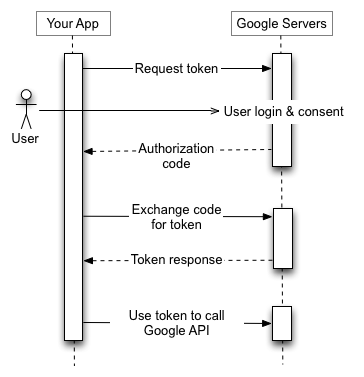
\includegraphics[width=8cm, keepaspectratio]{img/webflow}
	\caption{Esquema solicitud token para OAuth 2.0}
	\label{fig:OAuth}
\end{figure}
\begin{enumerate}
	\item \textbf{Obtener las credenciales de OAuth 2.0 desde la Consola de la API de Google,} que serán una ID y un \textit{client secret} conocidos tanto por Google como por la aplicación. Estas credenciales hay que descargarlas en un JSON, cuyo nombre necesitará la aplicación para los pasos posteriores.
	\item \textbf{Obtener un token de acceso del Servidor de Autorización de Google.} La aplicación realiza la solicitud del token al Servidor, que le devolverá el token preciso.
	\item \textbf{Enviar el token de acceso a la API a la que se desea acceder.} Una vez que la aplicación obtiene un token de acceso, lo envía a la API en un encabezado de autorización HTTP. 
	\item \textbf{Actualiza el token de acceso, si es necesario.} Los tokens de acceso tienen vidas limitadas, por lo que se puede obtener un token de actualización, que permitirá a la aplicación obtener nuevos tokens de acceso.
\end{enumerate}


\section{Pycountry}
\textit{pycountry}~\cite{pycountry:1} es un paquete que proporciona idioma, territorio, moneda y códigos de script de ISO de los países, así como sus traducciones entre ellos, tomados del paquete \textit{iso-codes}.\\

Se puede acceder a los países a través de un objeto de base de datos que ya está configurado al importar pycountry: \textit{\textbf{countries}}. Para acceder a un país específico, habrá que hacerlo con \textit{\textbf{get()}} (\textit{pycountry.countries.get(name=...)}).

\section{Pillow}
\textit{pillow}~\cite{pillow:1} es un \textit{fork} de PIL~\footnote{\url{https://pypi.org/project/PIL/}}. PIL es la Biblioteca de Imágenes de Python (Python Imaging Library) que agrega capacidades de procesamiento de imágenes a su intérprete de Python. Esta biblioteca es compatible con muchos formatos de archivo y proporciona un potente procesamiento de imágenes y capacidades gráficas.\\

En este proyecto se utiliza el método \textit{Image} de PIL~\footnote{\url{https://pillow.readthedocs.io/en/3.1.x/reference/Image.html}}, que se utiliza para representar una imagen. Proporciona funciones como cargar imágenes desde archivos, o crear nuevas imágenes.


\section{Pandas}

FIXME: ¿no usabas pandas para las gráficas? ¡Coméntalo aquí!

%%%%%%%%%%%%%%%%%%%%%%%%%%%%%%%%%%%%%%%%%%%%%%%%%%%%%%%%%%%%%%%%%%%%%%%%%%%%%%%%
%%%%%%%%%%%%%%%%%%%%%%%%%%%%%%%%%%%%%%%%%%%%%%%%%%%%%%%%%%%%%%%%%%%%%%%%%%%%%%%%
% DISEÑO E IMPLEMENTACIÓN %
%%%%%%%%%%%%%%%%%%%%%%%%%%%%%%%%%%%%%%%%%%%%%%%%%%%%%%%%%%%%%%%%%%%%%%%%%%%%%%%%

\cleardoublepage
\chapter{Diseño e implementación}
\label{chap:diseño}

\section{Arquitectura general}
\label{sec:arquitectura}
En la figura ~\ref{fig:esquema} se puede observar un esquema a modo de resumen del proceso que sigue el proyecto. A continuación, describiré cada bloque de este esquema.

\begin{figure}[h!]
	\centering
	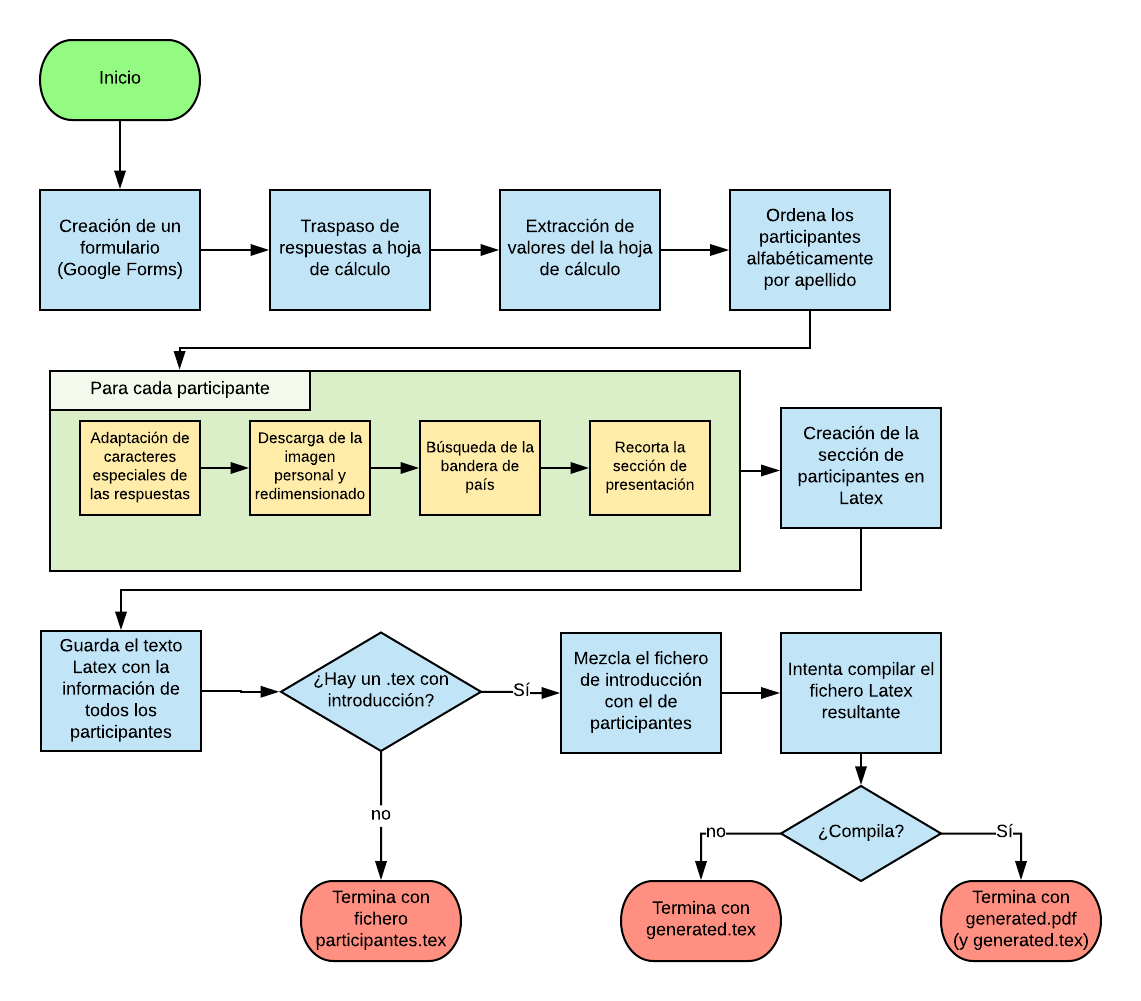
\includegraphics[width=12cm, keepaspectratio]{img/Esquema}
	\caption{Esquema de funcionamiento}
	\label{fig:esquema}
\end{figure}


\section{Creación de un formulario (Google Forms)}
\label{sec:formulario}
La base para obtener un buen resultado final, es crear desde el inicio un buen formulario. Para ello, hay que anticiparse a las respuestas de las personas que van a rellenar nuestra encuesta y, para esto, Google Forms nos ayuda mucho, ya que nos permite elegir entre múltiples tipos de respuestas posibles.\\

Por ejemplo, si preguntamos el nombre de la persona, elegiremos como tipo de respuesta la opción \textbf{Respuesta corta}, ya que el nombre consta de pocas palabras. En cambio, si pedimos una descripción, convendría elegir la opción \textbf{Párrafo} (incluso se puede limitar el número de caracteres de dicho párrafo). En los casos en los que conocemos de antemano las posibles respuestas de los asistentes, y éstas se vayan a repetir entre varios de ellos, podemos elegir las opciones de \textbf{Casillas de verificación}, \textbf{Selección múltiple} o \textbf{Desplegable}, según creamos conveniente. Algunos ejemplos de estos casos serían unas casillas de verificación para respuestas de Sí/No, o un desplegable para elegir la nacionalidad de la persona.\\

Con estos últimos casos, conseguiremos que todas las respuestas sean concisas y uniformes. Si no lo hacemos de esta forma y preguntamos, por ejemplo, ``¿Cuál es tu mes de nacimiento?'', dos personas distintas que hayan nacido en el mismo mes pueden contestar ``Yo nací en enero'' y ``Mi mes de nacimiento es enero''. Sin embargo, si aquí elegimos como tipo de respuesta un desplegable en el que simplemente haya que seleccionar el mes, obtendremos en ambas respuestas ``Enero''. Esto nos puede ayudar en el futuro si queremos, por ejemplo, buscar a todas las personas que tengan la misma respuesta a una determinada pregunta.\\

Además de estas, hay varias opciones más para las respuestas.

FIXME: faltaría un pantallazo del Google Forms


\section{Traspaso de respuestas a hoja de cálculo}
\label{sec:pasaraExcel}
Una vez que los participantes han rellenado el formulario, podemos acceder a sus respuestas de varias maneras: en la propia página de las preguntas, donde se pueden ver tanto las respuestas individuales como un resumen de las respuestas globales; y exportando las respuestas a una hoja de cálculo.\\

Realizaremos esta última opción, de manera que todos los datos quedarán volcados en una hoja de cálculo de Google. Esta hoja de cálculo tendrá la siguiente estructura:
\begin{itemize}
	\item En la primera fila aparece en cada celda una pregunta de las realizadas, a excepción de la primera celda, llamada ``Timestamp'', que indicará la fecha y hora a la que ha contestado cada participante.
	\item En cada una de las siguientes filas, aparecerá bajo cada pregunta la correspondiente respuesta de un participante.
\end{itemize}


\section{Extracción de los valores de la hoja de cálculo}
\label{sec:extraerExcel}
Esta es la primera parte que pertenece a mi proyecto. Lo primero que hace es obtener las credenciales necesarias para utilizar la API de Google Sheet. Una vez acreditado, con la URL de la hoja de cálculo que hemos obtenido del formulario, procedemos a la extracción de todos los datos. En este caso, no necesitamos la primera fila, donde aparecen los enunciados de las preguntas, por lo que indicaremos en el programa que queremos la información a partir de la celda 'A2'.\\

El resultado de este proceso será un array en el que cada elemento será otro array. Es decir, cada fila de la hoja de cálculo, se convertirá en un array cuyos elementos serán cada respuesta (cada celda). Estas filas (array) se guardan a su vez en otro array, quedando este último como un array de filas. Esta descripción se puede entender mejor con el siguiente ejemplo:

\begin{figure}[h!]
	\centering
	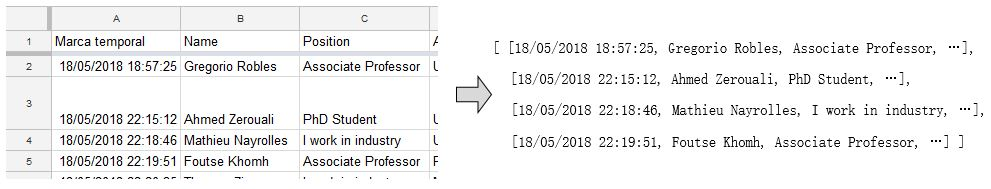
\includegraphics[width=17cm, keepaspectratio]{img/ejemplo45real}
	\caption{Ejemplo hoja de cálculo a array}
	\label{fig:ejemplo4_5}
\end{figure}

\subsection{Volcado de valores a NamedTuple}
\label{subsec:namedtuple}
Una vez tenemos el array con todos los datos, convertiremos este \textit{array de arrays} en un \textit{array de NamedTuples}.\\

NamedTuple es una \textit{``Tupla con nombre''}. Tiene una estructura parecida a la del array, pero cada elemento de éste se identifica con un nombre. Siguiendo el ejemplo anterior de la figura ~\ref{fig:ejemplo4_5}, el resultado sería:\\

\begin{figure}[h!]
	\centering
	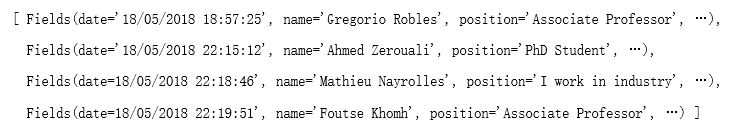
\includegraphics[width=17cm, keepaspectratio]{img/ejemplo45real2}
	\caption{Ejemplo NamedTuple}
	\label{fig:ejemplo4_5Namedtuple}
\end{figure}


En este caso, el NamedTuple se llama \textit{Fields}. Los nombres de los campos hay que definirlos antes de generar el NamedTuple. Una vez tenemos definido el NamedTuple, podemos referirnos a cada campo de éste con su nombre (si tuviésemos un array, tendríamos que saber en qué posición está el campo al que queremos referirnos para llamarlo). Por ejemplo, si del ejemplo anterior de la figura ~\ref{fig:ejemplo4_5Namedtuple} tenemos guardado el primer NamedTuple en una variable llamada \textit{row}, podremos acceder al nombre de la persona usando (\verb"row.name").

\section{Fichero de errores}
\label{sec:errores}
Durante la ejecución del programa, puede haber algún aspecto que no se consiga realizar, y se pueda realizar manualmente. Por ello, es conveniente informar al usuario de qué cosas no ha podido realizar el programa.\\

Al final de la ejecución, se generará también un fichero llamado \textbf{errors.txt} en el que aparecerán todos los errores que han ocurrido en la ejecución, así como el proceso para solventarlo manualmente.\\

En las siguientes secciones, se desarrollará más sobre los errores que se pueden dar en cada parte del programa.

\section{Proceso de tratamiento de información}
\label{sec:tratainfo}
Antes de generar el documento \LaTeX con la información que se ha extraído de la hoja de cálculo, hay que revisar toda esa información que tenemos, y ver si hay que hacer alguna modificación, o no usar literalmente el texto que tenemos en un campo.\\

Para esto, se utiliza un bucle que recorre los datos de todos los participantes. Este bucle tendría la siguiente estructura:

\begin{verbatim}
        order_by_name

        for row in fields:
            make_chars_latex_friendly
            download_image
            get_flag
            cut_presentation
    
            text_Latex = ...   
\end{verbatim}

La variable \textit{fields} es el array que contiene los datos de cada persona que ha rellenado la encuesta. Por tanto, en cada pasada del bucle la variable \textit{row} se corresponde con un NamedTuple, por lo que podremos extraer los datos con los nombres de los campos (\textit{row.name, row.affiliation}\ldots).\\

Exceptuando el proceso de ordenar alfabéticamente que se hace una única vez antes de entrar al bucle, los demás procesos se llevan a cabo para cada persona. Una vez tratada toda la información que poseemos, se generará el texto en \LaTeX.


\subsection{Ordenar alfabéticamente}
\label{subsec:orden}
Como en este caso tratamos con datos personales, hay que definir un orden de aparición, y para considerar a todos los participantes por igual, sin preferencias, ordenaremos a las personas alfabéticamente.\\

Para esto, en el método \textbf{\textit{order\_by\_name}} se extrae el apellido de cada nombre, y se guardan en un array. Este array es ordenado alfabéticamente con el método de Python \textit{sort}. Con la ayuda de un bucle y del array ordenado, se creará una nueva lista con todos los NamedTuples de datos ordenado alfabéticamente por el apellido del participante.


\subsection{Convertir caracteres especiales}
\label{subsec:especialCars}
Como la intención de este proyecto es generar un documento en \LaTeX, hay que adaptarlo para ello. \LaTeX tiene una serie de caracteres que utiliza para funciones especiales, tales como \textbackslash, \$, \%..., y para que al generar el PDF estos caracteres aparezcan correctamente, tienen que aparecer modificados en el documento \LaTeX.\\

Para solucionar este problema, se ha creado el método \textbf{\textit{make\_chars\_latex\_friendly}}, donde revisaremos todos los campos en busca de estos caracteres (\$, \#, \%, \&, \^, \_, \{, \}, \~ , \textbackslash) y cuando los encuentre, añadirá delante de ellos un \textit{backslash} (\textbackslash). De esta forma, aparecerá el carácter deseado, y no generará errores y confusiones a la hora de generar el PDF final.\\

Hay algunos casos especiales en los que no conviene hacer este proceso. Por ejemplo, si uno de los campos es una URL, y dicha URL no la vamos a escribir literalmente en el documento final, sino que la vamos a utilizar para obtener otro dato. En este caso tenemos, por ejemplo, un campo que corresponde a la URL de una imagen (se explicará a continuación), y esta URL será utilizada para descargar la imagen correspondiente, por tanto si hacemos el proceso anterior sobre la URL, cuando la utilicemos en el programa será incorrecta, por lo que no hay que modificarla.


\subsection{Descarga de imágenes personales}
\label{subsec:imagenes}
Una de las preguntas de nuestro formulario es para que se incluya una imagen personal, para añadirla junto a la información de cada asistente. En esta parte, cada asistente incluye una URL donde se encuentra su imagen, que habrá que descargar para poder incluirla en nuestro documento.\\

El método \textbf{\textit{download\_image}} se encarga de esto. Lo primero que hace es comprobar si la URL es una imagen: abre la URL con la librería urllib.request (\textit{resp = urllib.request.urlopen(url)}) y obtiene la información sobre ella (\textit{resp.info()}), que suele tener la siguiente apariencia:
\begin{verbatim}
        resp: Server: nginx/1.9.11
        Date: Tue, 19 Jun 2018 16:48:45 GMT
        Content-Type: image/jpeg;charset=UTF-8
        Transfer-Encoding: chunked
        Connection: close
        Content-Disposition: attachment; filename="paola_accioly.jpg"
        Cache-Control: max-age=604800
        Expires: Tue, 26 Jun 2018 16:48:45 GMT
        Strict-Transport-Security: max-age=31536000
\end{verbatim}

De toda esta información, el campo que nos interesa es el \textit{Content-Type}, ya que en él podremos comprobar si la URL es una imagen. Para extraer la información de este campo lo hacemos con \textit{resp.info().get('Content-Type')}.\\

Una vez que comprueba que este campo empieza por ``image\textbackslash'', se recoge también la extensión de la imagen, que aparece justo después de esta expresión (\textit{imgType}).A continuación, se procede a descargar la imagen con \textit{urllib.request.urlretrieve(url, nameImage)}. Esta expresión descarga la imagen de la URL que se indica en el primer parámetro de entrada, y la guarda con el nombre que aparece en el segundo parámetro.\\

El nombre de la imagen se compone de la ruta de la carpeta donde se va a guardar la imagen, seguido de la cadena ``img'' y un número identificador de cada persona, y acabando con la extensión que hemos almacenado anteriormente en \textit{imgType}.\\

Normalmente, las extensiones de las imágenes suelen ser las comunes .jpg, .png,\ldots, pero también pueden aparecer imágenes con extensión \textbf{.webp}. WebP es un formato de imagen creado por Google para reducir el tamaño de las imágenes y así disminuir el tiempo de carga de las mismas. Este formato no es reconocible por \LaTeX, por lo que hay que es necesario cambiar el formato de este tipo de imágenes, y para ello utilizamos \textit{im = Image.open(nameImage).convert("RGB")}. Ahora tenemos la imagen en el formato que queremos en la variable \textit{im}, por lo que hay que guardarla, por ejemplo, en .jpg, con \textit{im.save(nameImagejpg, "jpeg")}.\\

Además, se redimensionan las imágenes para que todas tengan el mismo tamaño y se genere un resultado uniforme.\\

En los casos en los que no se haya adjuntado URL de imagen, así como cuando haya algún problema para descargar la imagen (URL inexistente, URL no corresponde a una imagen, error en la descarga\ldots), se asignará una imagen por defecto que indica que no poseemos la imagen de esa persona. Además, en estos casos, se incluirá un mensaje de error para que el encargado de generar este documento pueda revisar manualmente estos casos.\\

Los mensajes de error en estas situaciones podrían ser de la siguiente manera:
\begin{verbatim}
-Error in image of Alberto Bacchelli (pos. 4) -> URL not found.
-Error in image of Safwat Hassan (pos. 26) -> There aren't URL.
-Error in image of Li Li (pos. 46) -> Download image manually
(change the name of the image in .tex).
\end{verbatim}
Aquí, nos indica en la imagen de qué participante nos ha saltado el error y la posición del documento donde aparece. En el caso en que haya que descargar la imagen manualmente, hay que cambiar en el documento \LaTeX el nombre de la imagen correspondiente (ya que al no poder descargarse se ha adjuntado la imagen por defecto). Para seguir las pautas de todo el proceso, convendría nombrar a la imagen como \textit{img} seguido del número de posición. En el caso del ejemplo el nombre sería \textit{img46}.\\

Finalmente, el método devolverá el nombre con el que se ha guardado la imagen de la persona correspondiente o, en su defecto, la imagen de error.


\subsection{Obtener banderas de nacionalidad}
\label{subsec:banderas}
Cada persona tendrá que indicar también su país de procedencia, y en vez de poner literalmente el nombre del país, se incluye una bandera de éste. Para ello tenemos una carpeta con todas las banderas guardadas cuyos nombres son el nombre del país en código \textit{``ISO 3166-1 alpha-2''}.\\

Para elegir la bandera correspondiente a cada persona, utilizamos el método \textbf{\textit{get\_flag}}, en el que se utiliza la librería \textit{pycountry} para convertir el nombre del país a código \textit{``ISO 3166-1 alpha-2''}. Para ello se obtiene la información de los códigos del país del cuál buscamos la bandera, con \textit{pycountry.countries.get(name=nationality)}, y nos quedaremos con el código en alpha-2.\\

Por ejemplo, si buscamos España:\\
\verb"nac = pycountry.countries.get(name='Spain')"

Obtendremos que \textit{nac} es:\\
\verb"Country(alpha_2='ES', alpha_3='ESP', name='Spain', numeric='724'," 
\verb"        official_name='Kingdom of Spain')"

Y nos interesaría quedarnos con el código alpha-2 en minúsculas:\\
\verb"nac.alpha_2.lower()"

De esta forma, añadiendo la extensión y, si fuera necesario, el directorio en el que se almacenan las imágenes de las banderas, se generaría el nombre de imagen \textit{flags/es.png}.\\

Al igual que con las imágenes, si ocurre algún error como que el país que buscamos no es correcto, se indicaría con un mensaje de error al usuario.

\subsection{Acortar presentaciones}
\label{subsec:presentacion}
Una de las partes del formulario consiste en una descripción personal. Debido a que es una pregunta de respuesta libre, la extensión de estas respuestas puede variar mucho. Como buscamos un resultado ordenado, no podemos permitir que una presentación que ocupe demasiado desordene nuestro trabajo, al ocupar, por ejemplo, el espacio que debería ocupar la información de otra persona.\\

Por ello, en el método \textbf{\textit{cut\_presentation}}, fijamos una longitud máxima para este campo, y si el texto escrito por el participante sobrepasa este valor, lo cortaremos e indicaremos que ha sido recortado añadiendo puntos suspensivos al final.


\section{Creación de la sección de participantes en \LaTeX}
\label{sec:creaParticipantes}
Una vez tenemos todos los datos listos, procedemos a desarrollar el texto en \LaTeX. El resultado final que buscamos tiene la siguiente estructura:
\begin{figure}[h!]
	\centering
	
\includegraphics[width=15cm, keepaspectratio]{img/esquemaLatex}
	\caption{Estructura información participante}
	\label{fig:ejemploLatex}
\end{figure}


\section{Apartados opcionales}
\label{sec:opcional}
Opcionalmente, se pueden añadir dos apartados más al documento.

\subsection{Diagramas de sectores}
\label{subsec:diagramas}
Con el método \textbf{\textit{generate\_graphs}} podemos obtener diagramas de sectores que indiquen el porcentaje de repetición de las respuestas que deseemos. Para ello, le pasamos como argumento un array con los nombres de los campos de los que queremos que se genere el diagrama. Estos nombres de campos se corresponden con los que indicamos anteriormente para el \textit{NamedTuple}.

\subsection{Listados de personas}
\label{subsec:listados}
Usando el método \textbf{\textit{generate\_list}} se puede crear una lista de todas las personas que han contestado \textit{``Sí''} a las preguntas que se pasarán como argumentos en la llamada al método. Una condición básica en este caso, es que las preguntas que indiquemos deben ser de respuesta \textit{Sí/No}. E igual que antes, para darle como argumento las preguntas que queremos, se hará con un array con los nombres del \textit{NamedTuple}.


\section{Guarda el fichero \LaTeX con los datos}
\label{sec:guardaLatex}
Cuando se ha formado el texto \LaTeX con los datos de todos los participantes, guardado en una variable, se procede a escribir este texto en un fichero .tex llamado \textbf{participants.tex}. En él aparecerá únicamente la sección de participantes. Si queremos incluir esta sección en otro documento \LaTeX (nos referiremos a él como \textit{principal}) podremos hacerlo añadiendo en este último documento el comando \mbox{\textit{\textbackslash input\{participants\}}}.\\

Así, en el documento principal podremos añadir una portada, unas páginas de introducción, formatos para el texto, cabeceras o pies de página, etc.\\

Con esto, al compilar el documento principal, obtendremos un PDF con la unión del documento principal y el de los participantes, que es el resultado deseado.


\section{Unir automáticamente documentos \LaTeX}
\label{sec:uneLatex}
El proceso de la sección anterior también se puede automatizar, es decir, en vez de tener dos documentos y que uno llame al otro, podemos unir los .tex. Para esto, necesitamos tener listo el documento principal al que nos referíamos antes, y que en él aparezca el comando \mbox{\textit{\textbackslash input\{participants\}}}. Este documento deberá llamarse \textbf{\textit{intro.tex}}\\

Nuestro programa buscará este fichero y leerá su contenido, buscando la sentencia \mbox{\textit{\textbackslash input\{participants\}}}, que será sustituida por el texto que hemos producido con los datos de los participantes. Una vez que tenemos la información de los participantes unida al texto del documento \textit{intro.tex}, lo guardaremos en un nuevo fichero, llamado \textbf{\textit{generated.tex}}, quedando todo el contenido en un único documento \LaTeX.\\

Si no se pueden unir los documentos, es decir, no se encuentra el fichero \textit{intro.tex} o la sentencia donde se introduce la información de los participantes, se mostrará un mensaje indicando que se ha creado el fichero con la sección de los participantes, así como su nombre, listo para incluirse en otro .tex:\\
\verb"        Participants section created (participants.tex). Include"\\
\verb"        it in your .tex"



\section{Compilado del documento \LaTeX}
\label{sec:compilado}
En caso de que hayamos conseguido obtener el documento \textit{generated.tex}, y contemos en nuestro PC con el paquete de \LaTeX instalado, el programa intentará compilarlo con el comando \textbf{\textit{xelatex generated.tex}} a través de una llamada al sistema:\\
\verb"        os.system('xelatex generated.tex')"\\

Si se ha compilado correctamente, obtendremos por pantalla un mensaje informativo indicando que el PDF ha sido generado, y su nombre:\\
\verb"        PDF has been generated --> generated.pdf"\\

En caso de que haya algún problema para compilar, nos mostrará un mensaje de error:\\
\verb"        Impossible to generate PDF automatically. You must"\\
\verb"        compile in Latex manually"


%%%%%%%%%%%%%%%%%%%%%%%%%%%%%%%%%%%%%%%%%%%%%%%%%%%%%%%%%%%%%%%%%%%%%%%%%%%%%%%%
%%%%%%%%%%%%%%%%%%%%%%%%%%%%%%%%%%%%%%%%%%%%%%%%%%%%%%%%%%%%%%%%%%%%%%%%%%%%%%%%
% RESULTADOS %
%%%%%%%%%%%%%%%%%%%%%%%%%%%%%%%%%%%%%%%%%%%%%%%%%%%%%%%%%%%%%%%%%%%%%%%%%%%%%%%%

\cleardoublepage
\chapter{Resultados}
\label{chap:resultados}
La mejor manera de mostrar los resultados en este caso, es con ejemplos. Esta aplicación ya ha sido puesta a prueba en 3 ocasiones, en escenarios reales.\\

Aunque se muestran los ejemplos completos en la sección \ref{app:ejemplos}, las siguientes imágenes muestran algunos fragmentos del resultado final.\\

\begin{itemize}
\item La primera prueba se realizó para el \textbf{\textit{15\raisebox{5pt}{th} International Conference on Mining Software Repositories (MSR) 2018}}\footnote{\url{https://conf.researchr.org/home/msr-2018}}, celebrada el 28 y 29 de mayo de 2018 en Gotemburgo (Suecia), y el resultado fue el mostrado en la figura \ref{fig:imgMSR}.
\begin{figure}[h!]
	\centering
	\fbox{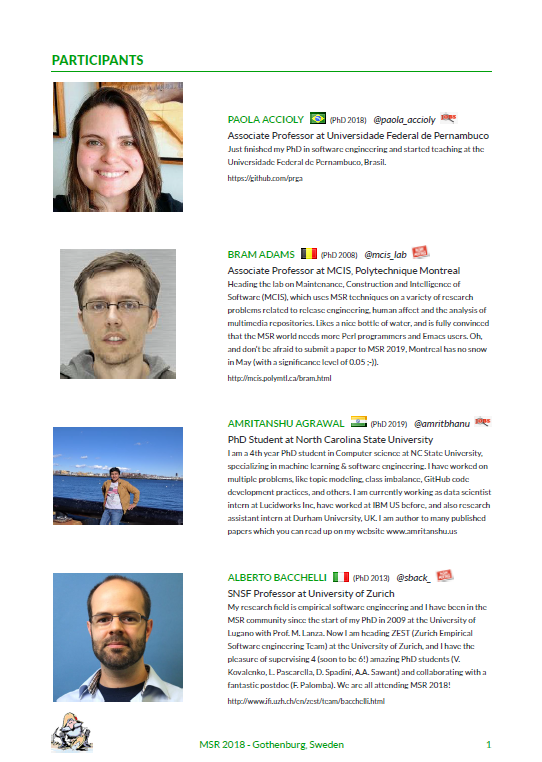
\includegraphics[width=15cm, keepaspectratio]{img/MSR}}
	\caption{Página ConfBook MSR 2018}
	\label{fig:imgMSR}
\end{figure}

\item La segunda ocasión en la que se ha utilizado la aplicación ha sido para el \textbf{\textit{14\raisebox{5pt}{th} International Conference on Open Source Systems (OSS) 2018}}\footnote{\url{https://www.oss2018.org/}}\footnote{\url{http://sattose.org/2018}}, celebrada del 8 al 10 de junio de 2018 en Atenas (Grecia). Este caso se muestra en la figura \ref{fig:imgOSS}.
\begin{figure}[h!]
	\centering
	\fbox{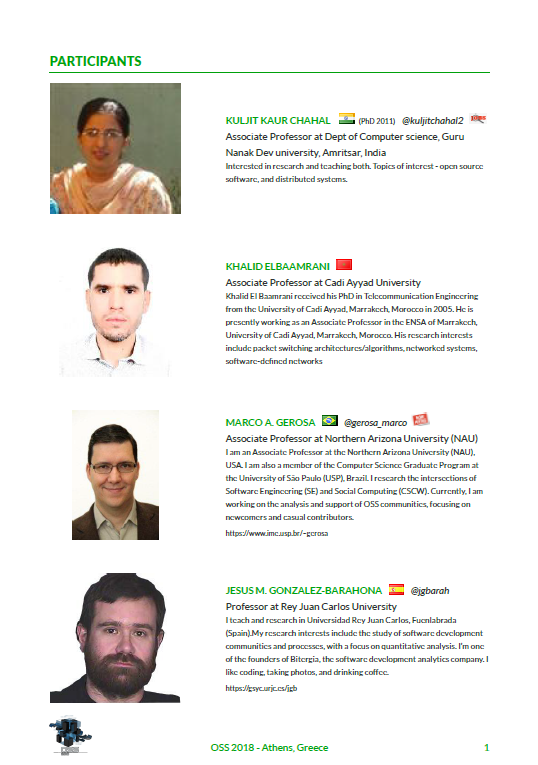
\includegraphics[width=15cm, keepaspectratio]{img/OSS}}
	\caption{Página ConfBook OSS 2018}
	\label{fig:imgOSS}
\end{figure}

\item El último caso en el que se ha usado es en el \textbf{\textit{11\raisebox{5pt}{th} Seminar on Advanced Techniques \& Tools for Sotware Evoluton SATToSE 2018}}, celebrado en Atenas (Grecia) del 4 al 6 de julio de 2018. Este ejemplo es el mostrado en el ejemplo \ref{fig:imgSATToSE}.
\begin{figure}[h!]
	\centering
	\fbox{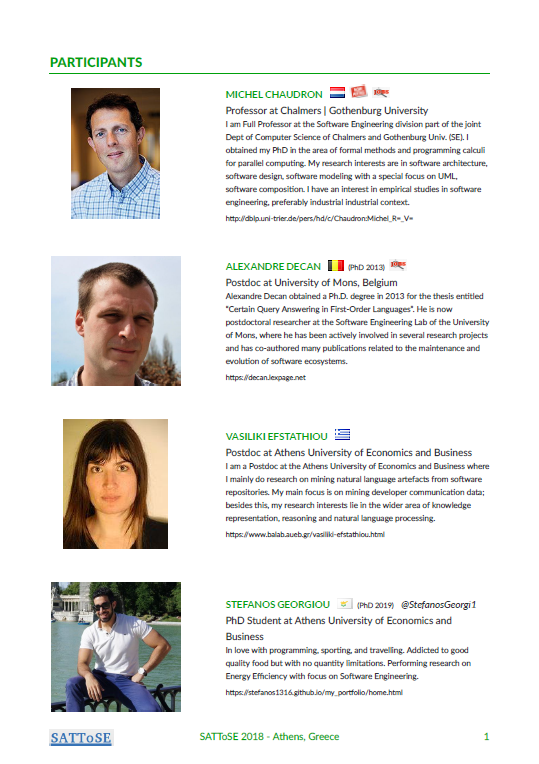
\includegraphics[width=15cm, keepaspectratio]{img/SATToSE}}
	\caption{Página ConfBook SATToSE 2018}
	\label{fig:imgSATToSE}
\end{figure}
\end{itemize}


%%%%%%%%%%%%%%%%%%%%%%%%%%%%%%%%%%%%%%%%%%%%%%%%%%%%%%%%%%%%%%%%%%%%%%%%%%%%%%%%
%%%%%%%%%%%%%%%%%%%%%%%%%%%%%%%%%%%%%%%%%%%%%%%%%%%%%%%%%%%%%%%%%%%%%%%%%%%%%%%%
% CONCLUSIONES %
%%%%%%%%%%%%%%%%%%%%%%%%%%%%%%%%%%%%%%%%%%%%%%%%%%%%%%%%%%%%%%%%%%%%%%%%%%%%%%%%

\cleardoublepage
\chapter{Conclusiones}
\label{chap:conclusiones}


\section{Consecución de objetivos}
\label{sec:consecucion-objetivos}
Al principio de esta memoria enumeré una serie de objetivos que pretendía conseguir a lo largo del proyecto, los cuales se analizan a continuación para comprobar si se han conseguido o no.

\begin{itemize}
  \item \textbf{Usar la aplicación para casos reales.} Como se ha indicado anteriormente en la sección de Resultados, este aplicación se ha utilizado en tres casos reales: \textit{MSR, OSS} y \textit{SATToSE}.
  \item \textbf{Sencillez de uso.} Para personas familiarizadas este campo, así como las tecnologías utilizadas, resultará fácil ejecutar el programa para la obtención del \textit{book}. Sin embargo, en el caso de las personas que no tengan ninguna relación con las tecnologías que se han utilizado, podría resultar difícil la ejecución.
\end{itemize}


\section{Aplicación de lo aprendido}
\label{sec:aplicacion}
A lo largo de la carrera he adquirido muchas habilidades y aprendizajes en diferentes áreas, siempre relacionadas con mi carrera de Ingeniería de Tecnologías de la Telecomunicación. De todas ellas, las que he podido aplicar en el desarrollo de este proyecto han sido:

\begin{enumerate}
  \item \textbf{La programación.} Aunque para mí era totalmente desconocida antes de llegar a la universidad, decidí hacer este Trabajo de Fin de Grado totalmente relacionado con ella, ya que ha sido lo que más me ha interesado de todo el grado, y a lo que me gustaría dedicarme. Las asignaturas que me han introducido a la programación y me han enseñado programación a bajo nivel han sido \textit{Fundamentos de la Programación, Programación de Sistemas de Telecomunicación} y \textit{Sistemas Operativos}.
  
  La programación a más alto nivel la he aprendido gracias a asignaturas como \textit{Servicios y Aplicaciones Telemáticas} o \textit{Ingeniería de Sistemas de Telecomunicación}.
  \item \textbf{Capacidad de trabajar bajo presión y enfrentamiento a los problemas.} A lo largo de la carrera nos enfrentamos a numerosos casos en los que tenemos que trabajar bajo presión, como en épocas de exámenes, en las que tenemos varios exámenes en muy pocos días, teniendo en nuestra mente la obligación de aprobarlos todos. Además, esta carrera me ha enseñado, y no en asignaturas, que debemos enfrentarnos a los problemas y buscar la manera de resolverlos.
\end{enumerate}


\section{Lecciones aprendidas}
\label{sec:lecciones_aprendidas}
Una de las cosas más importantes que he aprendido con este trabajo ha sido planificar un proyecto de gran envergadura como es este, y organizarlo tanto temporal como estructuralmente.\\

También he adquirido conocimientos en aplicaciones y tecnologías antes desconocidas para mí, como pueden ser \textit{Google Forms} o \textit{Google Sheet API}, que me han sido de gran ayuda en este proyecto, ya que me han permitido poder trabajar con los datos de manera online, sin tener que descargar y tratar documentos en local.\\

También he podido aprender mucho más sobre el lenguaje \LaTeX, del cual sabía muy poco antes de este trabajo. Además de utilizarlo en el programa para generar el book final, lo he utilizado para realizar esta memoria, y me han sido muy útiles los conocimientos adquiridos para ello.\\

Por último, y no menos importante, la realización de este proyecto, que he llevado a cabo a lo largo del curso, lo que incluye las épocas de mayor carga de trabajo como son los exámenes, unido a la realización de las prácticas curriculares, me ha enseñado a compaginar grandes cargas de trabajo para conseguir el mayor objetivo personal que tengo en este momento: la finalización del grado.


\section{Trabajos futuros}
\label{sec:trabajos_futuros}
Un posible trabajo futuro es crear una aplicación web en la que el gestor del seminario pueda crear de manera fácil un formulario y que cada persona lo rellene con sus datos. Así, automáticamente, se añadirían esos datos a los de los demás participantes y se generaría el pdf con la nueva incorporación.\\

También podría haber en esta misma web un apartado donde consultar de forma online los datos de los participantes que hayan rellenado el formulario, con enlaces a sus páginas personales.\\

De esta forma, se podría cumplir uno de los objetivos que no he conseguido cumplir en este proyecto: hacer que el proceso de generación del book lo puedan realizar personas que no tienen conocimientos sobre las tecnologías utilizadas, o no estén nada familiarizadas con este campo.\\

Otra idea es, además de la web, hacer una aplicación móvil, de manera que en vez de tener el documento en versión papel, se pueda tener toda la información en la app.






%%%%%%%%%%%%%%%%%%%%%%%%%%%%%%%%%%%%%%%%%%%%%%%%%%%%%%%%%%%%%%%%%%%%%%%%%%%%%%%%
%%%%%%%%%%%%%%%%%%%%%%%%%%%%%%%%%%%%%%%%%%%%%%%%%%%%%%%%%%%%%%%%%%%%%%%%%%%%%%%%
% APÉNDICE(S) %
%%%%%%%%%%%%%%%%%%%%%%%%%%%%%%%%%%%%%%%%%%%%%%%%%%%%%%%%%%%%%%%%%%%%%%%%%%%%%%%%

\cleardoublepage
\appendix
\chapter{Manual de usuario}
\label{app:manual}
Para que la aplicación funcione correctamente, es necesario tener instalado \textbf{\textit{Python 3}} o superior, además de los siguientes paquetes, en las versiones indicadas:
\begin{itemize}
	\item \textbf{\textit{google-api-python-client}}\cite{google_api_client:1} versión 1.6.5 o superior.
	\item \textbf{\textit{pycountry}}~\footnote{\url{https://pypi.org/project/pycountry/}} versión 18.2.23 o superior.
	\item \textbf{\textit{pillow}}\cite{pillow:1} versión 5.1.0 o superior.
	\item \textbf{\textit{oauth2client}}~\footnote{\url{https://pypi.org/project/oauth2client/}} versión 4.1.2 o superior.
\end{itemize}

Además, para conseguir el compilado en \LaTeX y que en la misma ejecución nos genere el documento en PDF, necesitamos tener instalado también \textbf{\textit{latex-xetex}} en la versión 3 o superior.\\

Una vez instalado todo lo anterior, tenemos que ejecutar el programa. Para hacerlo desde una \textit{Shell Unix} hay que ejecutar el comando \verb"python3 creator.py". Si todo va bien, al finalizar obtendremos en la carpeta de destino tanto los ficheros \LaTeX como el PDF con el resultado final.

\section{Dónde descargar la aplicación}
\label{sec:descarga_aplicacion}
El programa está disponible en el repositorio de GitHub:\\
\url{https://github.com/SheilaOM/TFG}


\cleardoublepage
\chapter{Ejemplo de uso}
\label{app:ejemplos}
Como he indicado con anterioridad, este proyecto se ha utilizado en casos reales, y los resultados han sido los siguientes.

\newpage
\section{15\raisebox{5pt}{th} International Conference on Mining Software Repositories (MSR) 2018}
\label{MSR}
\includepdf[pages=-]{2018-MSR-Confbook}


\section{14\raisebox{5pt}{th} International Conference on Open Source Systems (OSS) 2018}
\label{OSS}
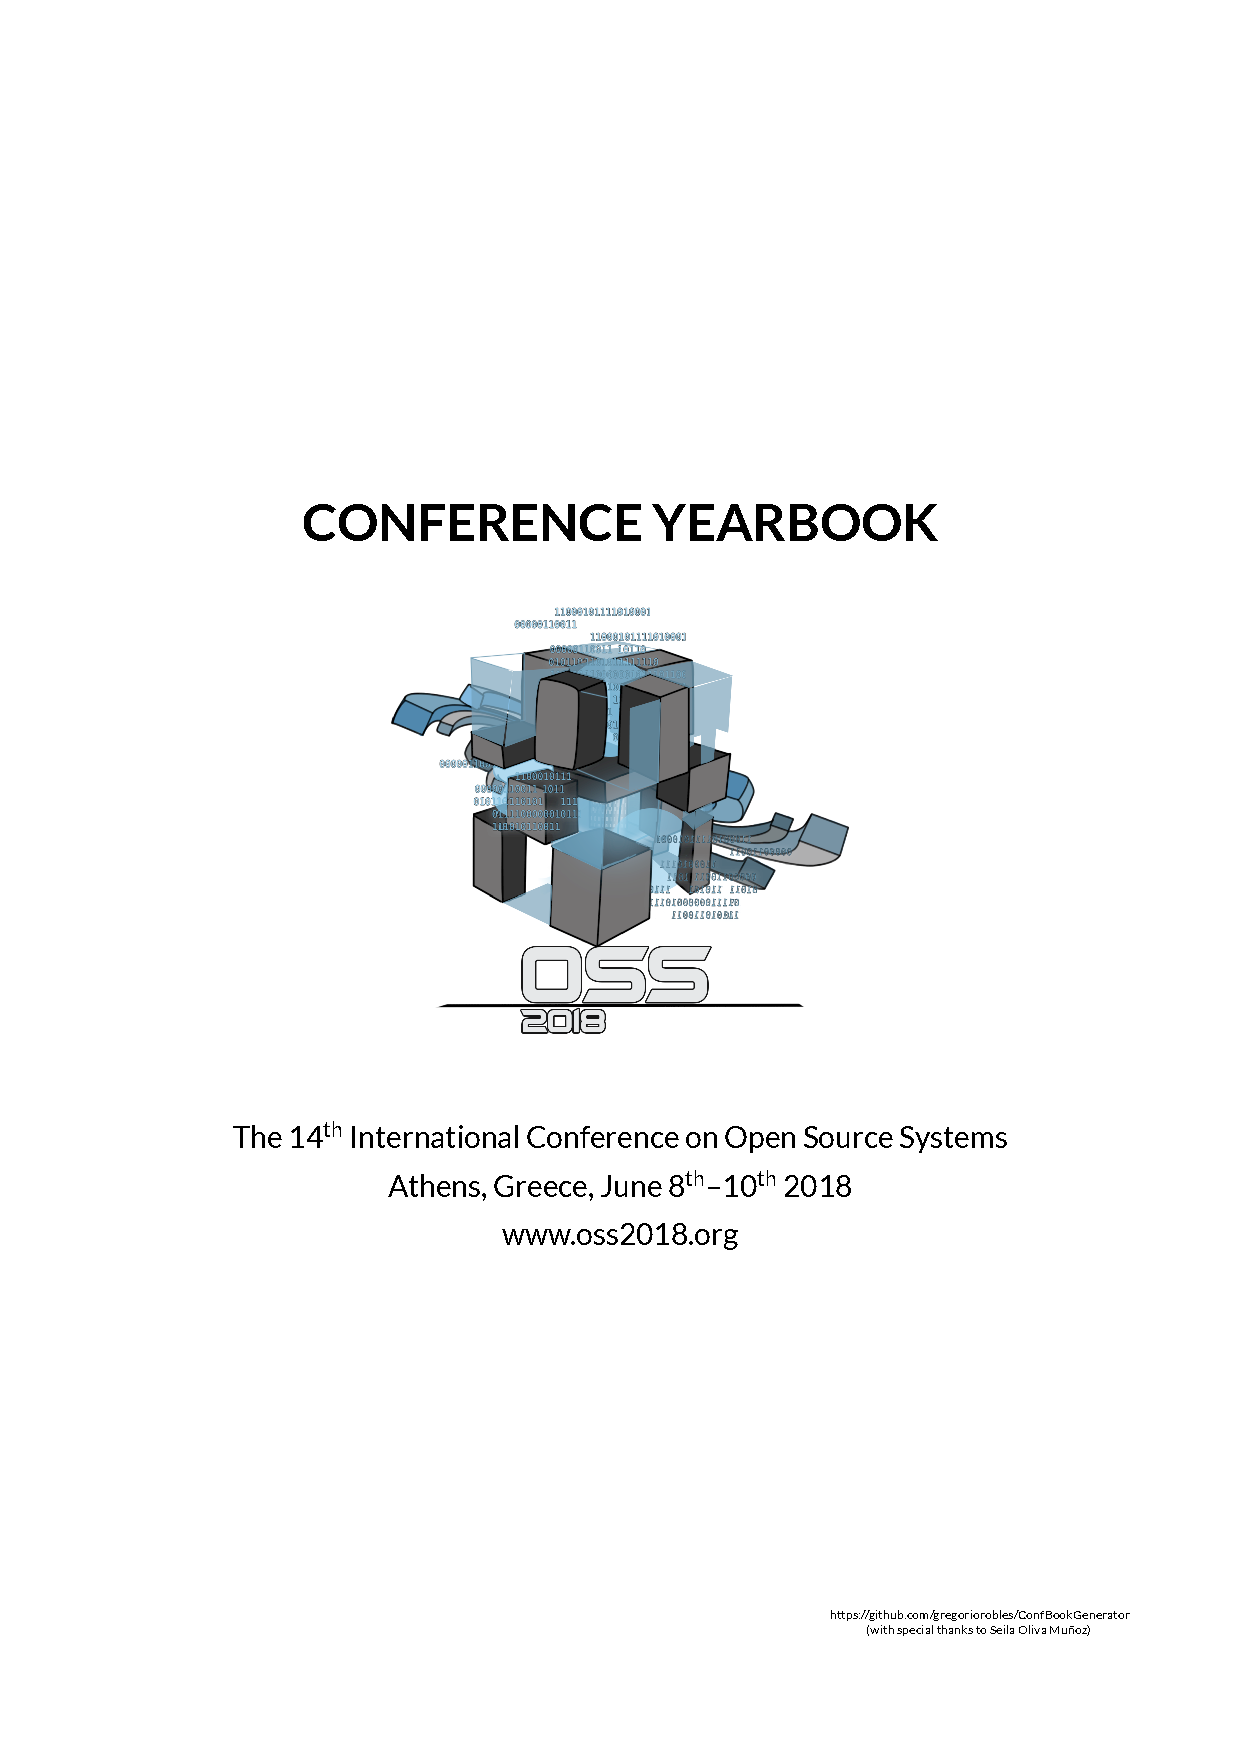
\includepdf[pages=-]{2018-OSS-Confbook}


\section{11\raisebox{5pt}{th} Seminar on Advanced Techniques \& Tools for Sotware Evoluton SATToSE 2018}
\label{SATToSE}

\includepdf[pages=-]{2018-SATToSE-Confbook}


%%%%%%%%%%%%%%%%%%%%%%%%%%%%%%%%%%%%%%%%%%%%%%%%%%%%%%%%%%%%%%%%%%%%%%%%%%%%%%%%
%%%%%%%%%%%%%%%%%%%%%%%%%%%%%%%%%%%%%%%%%%%%%%%%%%%%%%%%%%%%%%%%%%%%%%%%%%%%%%%%
% BIBLIOGRAFIA %
%%%%%%%%%%%%%%%%%%%%%%%%%%%%%%%%%%%%%%%%%%%%%%%%%%%%%%%%%%%%%%%%%%%%%%%%%%%%%%%%

\cleardoublepage

% Las siguientes dos instrucciones es todo lo que necesitas
% para incluir las citas en la memoria
%\bibliographystyle{abbrv}
\bibliographystyle{unsrt}

\bibliography{memoria}  % memoria.bib es el nombre del fichero que contiene
% las referencias bibliogríficas. Abre ese fichero y mira el formato que tiene,
% que se conoce como BibTeX. Hay muchos sitios que exportan referencias en
% formato BibTeX. Prueba a buscar en http://scholar.google.com por referencias
% y verás que lo puedes hacer de manera sencilla.
% Más información:
% http://texblog.org/2014/04/22/using-google-scholar-to-download-bibtex-citations/

\end{document}
